\documentclass[12pt]{article}
\usepackage[english]{babel}
\usepackage[utf8]{inputenc}
\usepackage[T1]{fontenc}
\usepackage{amsmath}
\usepackage{graphicx}
\usepackage[colorinlistoftodos]{todonotes}
\usepackage{listings}
\usepackage{enumitem}
\usepackage{listingsutf8}
\usepackage{xparse}
\usepackage[hmargin=2cm]{geometry}
\usepackage{color} 
\NewDocumentCommand{\codeword}{v}{%
\texttt{\textcolor{blue}{#1}}%
}
\definecolor{codegreen}{rgb}{0,0.6,0}
\definecolor{codegray}{rgb}{0.5,0.5,0.5}
\definecolor{codepurple}{rgb}{0.58,0,0.82}
\definecolor{backcolour}{rgb}{0.95,0.95,0.92} 
\lstdefinestyle{mystyle}{
    backgroundcolor=\color{backcolour},   
    commentstyle=\color{codegreen},
    keywordstyle=\color{magenta},
    numberstyle=\tiny\color{codegray},
    stringstyle=\color{codepurple},
    basicstyle=\footnotesize,
    breakatwhitespace=false,         
    breaklines=true,                 
    captionpos=b,                    
    keepspaces=true,                 
    numbers=left,                    
    numbersep=5pt,                  
    showspaces=false,                
    showstringspaces=false,
    showtabs=false,                  
    tabsize=2
}
\lstset{style=mystyle}
\lstset{inputencoding=utf8/latin1}
%Para mostrar el código bonito 
\lstset{language=C++} 
\lstdefinestyle{customc}{
  belowcaptionskip=1\baselineskip,
  breaklines=true,
  frame=L,
  xleftmargin=\parindent,
  language=C++,
  showstringspaces=false,
  basicstyle=\footnotesize\ttfamily,
  keywordstyle=\bfseries\color{green!40!black},
  commentstyle=\itshape\color{purple!40!black},
  identifierstyle=\color{blue},
  stringstyle=\color{orange},
}

\begin{document}
\begin{titlepage}
\newcommand{\HRule}{\rule{\linewidth}{0.5mm}}
\center
\textsc{\LARGE Universidad de Granada}\\[1.5cm] % Name of your university/college
\textsc{\Large Algorítmica}\\[0.5cm] % Major heading such as course name
\HRule \\[0.4cm]
{ \huge \bfseries Práctica 4: Backtracking}\\[0.4cm] % Title of your document
\HRule \\[1.5cm]
\begin{minipage}{0.4\textwidth}
\begin{flushleft} \large
\emph{Autora:}\\
Elena Merelo Molina \textsc{} % Your name
\end{flushleft}
\end{minipage}
~
\begin{minipage}{0.4\textwidth}
\begin{flushright} \large
\emph{} \\
\textsc{} % Supervisor's Name
\end{flushright}
\end{minipage}\\[2cm]
{\large Mayo de 2018}\\[2cm] % Date, change the \today to a set date if you want to be precise

\includegraphics[scale=0.5]{./logo.jpg}
\vfill % Fill the rest of the page with whitespace
\end{titlepage}


\section{Problema a resolver}
Se va a celebrar una cena de gala a la que asistirán n invitados. Todos se van a sentar alrededor de una única
gran mesa rectangular, de forma que cada invitado tendrá sentados junto a él a otros dos comensales (uno a
su izquierda y otro a su derecha). En función de las características de cada invitado (por ejemplo categoría
o puesto, lugar de procedencia,...) existen unas normas de protocolo que indican el nivel de conveniencia de
que dos invitados se sienten en lugares contiguos (supondremos que dicho nivel es un número entero entre
0 y 100). El nivel de conveniencia total de una asignación de invitados a su puesto en la mesa es la suma
de todos los niveles de conveniencia de cada invitado con cada uno de los dos invitados sentados a su lado.
Se desea sentar a los invitados de forma que el nivel de conveniencia global sea lo mayor posible. Diseñar
e implementar un algoritmo vuelta atrás para resolver este problema. Realizar un estudio empírico de su
eficiencia.

\section{Explicación de mi solución}
Para resolver el problema he creado la clase \verb|matriz_de_conveniencia|, en la que agrupamos todos los métodos y atributos necesarios. Veámoslos uno a uno.

\begin{itemize}[wide, nosep, labelindent = 0pt, topsep = 1ex]
\item[\textbf{Atributos privados}]
\item \verb|vector<vector<int> > m| Es la matriz que contiene los niveles de conveniencia entre los invitados a la cena (de esta manera, por ejemplo $m[0][1]$ contiene el nivel de conveniencia del invitado 0 al 1, y así).
\item \verb|vector<int> solucion| vector con el orden en el que han de sentarse los invitados para que el nivel de conveniencia total sea máximo.
\end{itemize}
\begin{itemize}[wide, nosep, labelindent = 0pt, topsep = 1ex]
\item[\textbf{Métodos públicos}] 
\item Constructor de la matriz de conveniencia a partir de un tamaño n pasado como parámetro, rellena las componentes de la misma con un número aleatorio entre 0 y 100.
\begin{lstlisting}
matriz_de_conveniencia(int n){
    int i, j;
    //Inicializamos la semilla para generar los números aleatorios
    srand(time(NULL));
  
    m.resize(n);

    for(i= 0; i< n; i++)
      m[i].resize(n);

    for(i= 0; i< n ; i++)
      for(j= 0; j< n; j++)
        m[i][j]= i != j? rand() % 100: 0; //el número generado es un entero entre 0 y 100

  }
\end{lstlisting}

\item Método que devuelve el vector solución:
\begin{lstlisting}
vector<int> get_solucion(){
  return solucion;
}
\end{lstlisting}

\item Método que calcula el nivel de conveniencia total para un vector dado:
\begin{lstlisting}
  int conveniencia_total(vector<int> v){
    int sum= 0, n= v.size();

    for(int i= 1; i<n-1; i++)
      sum+=m[ v[i] ][ v[i+1] ] + m[ v[i] ][ v[i-1] ];

    sum+=m[ v[n-1] ][ v[n-2] ] + m[ v[n-1] ][ v[0] ];
    sum+=m[ v[0] ][ v[1] ] + m[ v[0] ][ v[n-1] ];

    return sum;
  }
\end{lstlisting}
El algoritmo es simple; para cada elemento del vector v pasado como parámetro, que consideramos como invitados, obtiene la conveniencia con el invitado de la izquierda y el de la derecha, y las suma al total. No obstante, hay que tener en especial consideración el primer y último elemento del vector, por eso los tenemos fuera del bucle: a la izquierda de $v[0]$ está $v[n-1]$ y viceversa, esto es lo que se expresa en las dos últimas líneas. Con un ejemplo queda más claro: Supongamos que tenemos cuatro invitados, n= 4. Entonces empezamos desde el invitado 1 y vemos la conveniencia con 2 y 0, son su izquierda y derecha, y una vez visto esto nos movemos a la persona 2. Sumamos la conveniencia de 2 con 1 y con 3 y nos movemos a 3, mirando la conv con 2 y con 4. De esta manera, iteramos desde 1 hasta n-1. Una vez hecho esto habremos de añadir la conveniencia de 0 con 1 y 0 con el último comensal, así como la de 4 con 3 y 4 con 0. 

\item Método que comprueba si un invitado ha sido ya considerado:
\begin{lstlisting}
bool sentado(vector<int> v, int x){
    return count(v.begin(), v.end(), x) == 1;
  }
\end{lstlisting}

\item Método que calcula el vector complementario a uno pasado como parámetro dentro de la matriz de conveniencia, esto es, si nos pasan un vector con tres invitados y en total a la cena de gala van seis, este método devolvería un vector con los invitados de la cena que no están en el vector inicial:
\begin{lstlisting}
  vector<int> complementario(vector<int> v, int n){
    vector<int> result;
    for(int i= 0; i< n; i++)
      if(!sentado(v, i))
        result.push_back(i);

    return result;
  
\end{lstlisting}

\item Algoritmo de backtracking propiamente dicho que calcula el máximo nivel de conveniencia: 
\begin{lstlisting}
  int max_nivel_conv(vector<int> v){
    int max_conv= 0, conv= 0;
    vector<int> por_sentar= complementario(v, m.size());

    for(int i= 0; i< por_sentar.size(); i++){
      v.push_back(por_sentar[i]);

      conv= conveniencia_total(v);

      if(conv > max_conv){
        max_conv= conv;
        solucion= v;
        max_nivel_conv(v);
      }

      v.pop_back();
    }
    return max_conv;
  }
\end{lstlisting}
Su funcionamiento no es muy complejo: calcula las permutaciones sin repetición de los n invitados, obteniendo la conveniencia de esa combinación y va comparando con la máxima de ellas, de manera que al final ésta es la que devuelve.
\end{itemize}

\section{Eficiencia empírica}
Para hallarla empleamos la librería \verb|time.h|. Tenemos el siguiente \verb|main|: 
\begin{lstlisting}
/*
#include "matriz_de_conveniencia.cpp"
using namespace std;

int main(int argc, char **argv){
  struct timespec cgt1, cgt2;
  double ncgt;  //para tiempo de ejecucion

  if(argc != 2){
    cout << "\nNumero de argumentos incorrecto";
    exit(-1);
  }

  int n= atoi(argv[1]), max_conv;
  matriz_de_conveniencia m(n);
  vector<int> v, f;

  clock_gettime(CLOCK_REALTIME, &cgt1);
  max_conv=  m.max_nivel_conv(v);
  clock_gettime(CLOCK_REALTIME, &cgt2);

  //cout << "\nEl maximo nivel de conveniencia es: " << max_conv;
  f= m.get_solucion();
  //cout << "\nPara ello los invitados han de estar sentados en el orden: ";
  for(int i= 0; i< f.size(); i++)
    // cout << f[i] << " ";

  ncgt= (double)(cgt2.tv_sec - cgt1.tv_sec) + (double) ((cgt2.tv_nsec - cgt1.tv_nsec) / (1.e+9));
  cout << "\n" << ncgt; //tiempo de ejecucion
}
\end{lstlisting}
Están comentadas las líneas que no son relativas al tiempo de ejecución para que a la hora de recoger todos los datos y dibujarlos sea más sencillo. Luego ponemos en marcha un script que ejecuta el main desde n=1 hasta 15, incrementando de 1 en 1 (ya para el tamaño 16 tardaba demasiado) y guarda los tiempos en un fichero:
\begin{lstlisting}
#!/bin/csh
@ inicio = 0
@ fin = 15
@ incremento = 1
@ i = $inicio
echo > tiempos_backtracking.dat
while ( $i <= $fin )
  echo Ejecucion tam = $i
  echo `../bin/main $i` >> tiempos_backtracking.dat
  @ i += $incremento
end
\end{lstlisting}

Comparando con diferentes funciones, vemos cómo es la obtenida, que no se puede aproximar bien por ninguna de ellas y da un salto muy grande del valor 14 al 15, al ser de orden O(n!):
\begin{figure}[h]
	\centering
	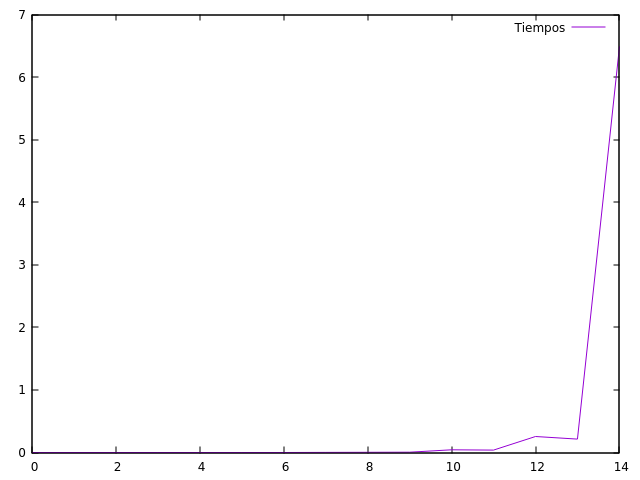
\includegraphics[scale=0.5]{../images/tiempos.png}
	\caption{Eficiencia empírica del algoritmo}
	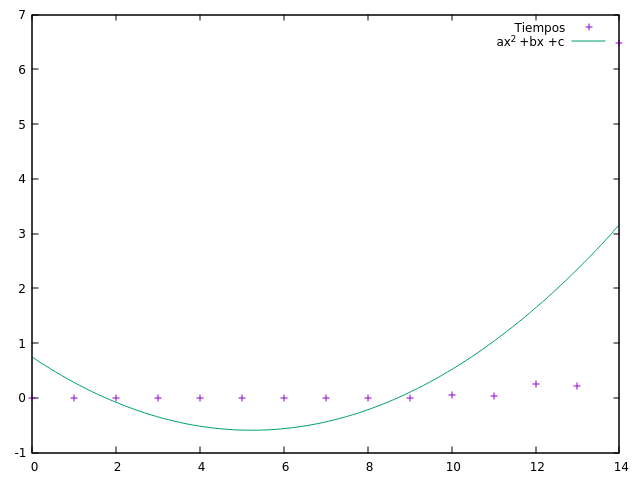
\includegraphics[scale=0.5]{../images/cuadratica.png}
	\caption{Gráfica del algoritmo comparada ajustada a una función cuadrática}
	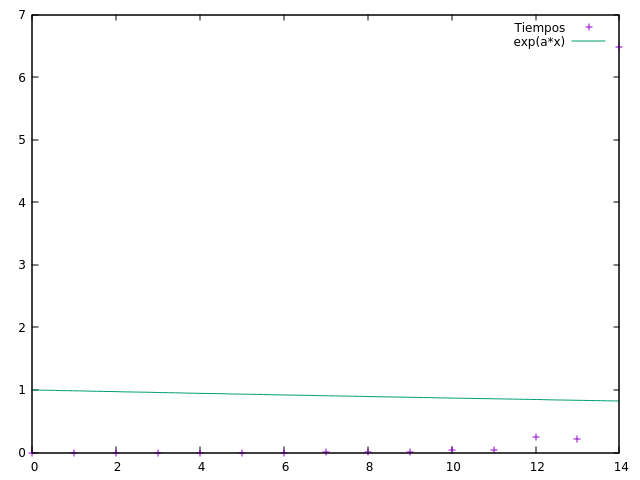
\includegraphics[scale=0.5]{../images/exp_plot.png}
	\caption{Algoritmo comparado con una exponencial}
		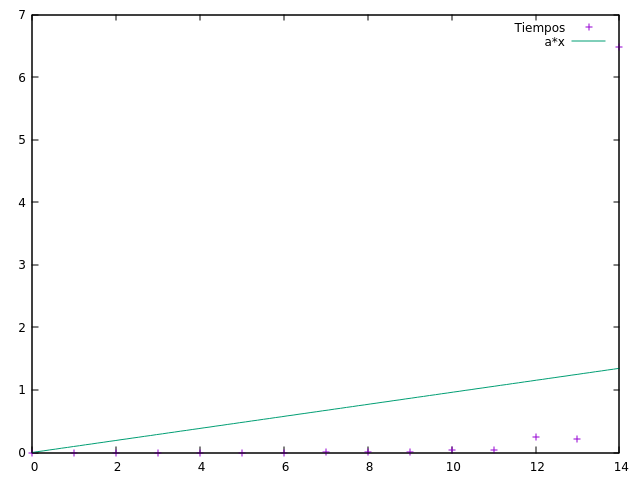
\includegraphics[scale=0.5]{../images/lineal_plot.png}
	\caption{Algoritmo comparado con una función lineal}
\end{figure}
\end{document}